\documentclass[9pt, landscape, a4paper]{article}

\usepackage{fontspec}
\renewcommand{\normalsize}{\fontsize{9}{11}\selectfont}
\usepackage[english]{babel}
\babelfont{rm}{Noto Sans}
\babelfont{sf}{Noto Sans}

\usepackage{amsmath}
\usepackage{amssymb}
\usepackage{hyperref}
\usepackage{url}
\usepackage{graphicx}
\usepackage{geometry}
\usepackage{enumitem}
\usepackage{parskip}
\usepackage{chemfig}
\usepackage{pdfpages}
\usepackage{xcolor}
\usepackage{tikz}
\usepackage{fancybox}
\usepackage{makecell}
\usepackage{pgfplots}
\usepackage{ulem}
\usepackage{wrapfig}
\usepackage{subcaption}
\usepackage{esvect}
\usepackage{siunitx}
\usepackage{mathtools}
\usepackage{varwidth}
\usepackage{multicol}
\usepackage{titlesec}
\usepackage{bm}
\usepackage{forest}
\usepackage{upgreek}
\usepackage{tabularx}
\usepackage{colortbl}
\usepackage[column=O]{cellspace}
\usepackage{tcolorbox}
\usepackage{siunitx}

\usetikzlibrary{arrows, arrows.meta}
\usetikzlibrary{decorations.pathreplacing}
\usetikzlibrary{decorations.markings}
\usetikzlibrary{patterns}
\pgfplotsset{compat=1.18}
\definecolor{darkgreen}{rgb}{0.0, 0.6, 0.0}
\DeclareMathOperator\arctanh{arctanh}

% ============= TABLE COLORS =============
\definecolor{col1}{RGB}{80,60,160}
\definecolor{col2}{RGB}{40,140,60}
\definecolor{col3}{RGB}{50,80,180}
\definecolor{col4}{RGB}{200,100,0}
\definecolor{headerblue}{RGB}{220,230,245}
\definecolor{headertxt}{RGB}{40,60,120}
\definecolor{notebg}{RGB}{255,248,220}
\definecolor{noteborder}{RGB}{200,160,0}

% ============= GEOMETRY =============
\geometry{
    a4paper,
    landscape,
    left=0.5cm,
    right=0.5cm,
    top=1.5cm, 
    bottom=0.5cm,
    footskip=0cm
}

\setlist{nosep, leftmargin=*}

\AtBeginDocument{
  \setlength{\abovedisplayskip}{3pt}
  \setlength{\belowdisplayskip}{3pt}
  \setlength{\abovedisplayshortskip}{0pt}
  \setlength{\belowdisplayshortskip}{0pt}
}

% ============= HEADER & TITLES =============
\usepackage{fancyhdr}
\pagestyle{fancy}
\fancyhf{}
\rhead{\small \vspace*{.1cm}Thermo and Fluid Dynamics Simulation Cheatsheet}
\lhead{\small \vspace*{.1cm}Matteo Frongillo}
\cfoot{\small \vspace*{.4cm}\thepage}
\cfoot{\small \vspace*{.4cm}\thepage/10}
\renewcommand{\headrulewidth}{0pt}
\setlength{\headsep}{4pt}

\titlespacing*{\part}{0pt}{6pt}{1pt}
\titlespacing*{\section}{0pt}{6pt}{1pt}
\titlespacing*{\subsection}{0pt}{6pt}{1pt}
\titlespacing*{\subsubsection}{0pt}{6pt}{1pt}

\titleformat{\part}{\large\bfseries\color{black}}{\thepart.}{0.4em}{}
\titleformat{\section}{\bfseries\color{red!80}}{}{0em}{}
\titleformat{\subsection}{\small\bfseries\color[HTML]{007AFF}}{}{0em}{}
\titleformat{\subsubsection}{\small\bfseries\color[HTML]{007355}}{}{0em}{}

% ============= META DATA =============
\newcommand{\pdftitle}[1]{\hypersetup{
  colorlinks=true,
  linkcolor=black,
  urlcolor=blue,
  pdftitle={#1},
  pdfauthor={Matteo Frongillo}
}}

% ============= RENEW COMMANDS =============

\makeatletter
\renewcommand{\author}[1]{%
  \def\@author{%
    #1\\
    \parbox{\textwidth}{%
      \centering
      \small Last update: \today
    }
  }%
}
\makeatother

\let\emptyset\varnothing

\makeatletter
\pgfmathdeclarefunction{arctan}{1}{%
    \begingroup
    \pgfmathparse{rad(atan(#1))}%
    \endgroup
}
\makeatother

\renewcommand{\tau}{\uptau}
\renewcommand{\nu}{\upnu}

% ============= NEW COMMANDS =============

\newcommand{\figbox}[1]{ 
  \begin{center}
    \fbox{\begin{varwidth}{\textwidth} #1 \end{varwidth}} 
  \end{center}       
}

\newcommand{\wrapfill}{
    \par
    \ifnum \value{WF@wrappedlines} > 0
        \addtocounter{WF@wrappedlines}{-1}%
        \null\vspace{
            \arabic{WF@wrappedlines}
            \baselineskip
        }
        \WFclear
    \fi
    \phantom{}
}

\ExplSyntaxOn
\DeclareDocumentCommand{\integral}{d[] d[] d[] d[]}
{
    \IfNoValueTF{#3}{
        \IfNoValueTF{#4}{
            \displaystyle \int #1\,d#2
        }{
            \text{Error: either 2 or 4 arguments must be provided}
        }
    }{
        \IfNoValueTF{#4}{
            \text{Error: either 2 or 4 arguments must be provided}
        }{
            \displaystyle
            \int\limits
                \IfNoValueF{#1}{\c_math_subscript_token{#1}}
                ^{\IfNoValueTF{#2}{}{#2}}
                #3\, d#4
        }
    }
}
\ExplSyntaxOff

\newcommand*\circled[1]{\tikz[baseline=(char.base)]{
            \node[shape=circle,draw,inner sep=1pt] (char) {\small #1};}}

\makeatletter
\newcommand*{\rom}[1]{\expandafter\@slowromancap\romannumeral #1@}
\makeatother

\makeatletter
\newcommand{\shorteq}{\mathrel{\mkern0.2mu\mathpalette\shorteq@\relax\mkern0.2mu}}
\newcommand{\shorteq@}[2]{\scalebox{0.5}[1]{$\m@th#1=$}}

\newcommand{\longeq}[1]{\mathrel{\mathpalette\longeq@{#1}}}
\newcommand{\longeq@}[2]{%
  \begingroup
  \sbox\z@{$\m@th#1=$}%
  \ifdim#2<\wd\z@
    \resizebox{#2}{\height}{\box\z@}%
  \else
    \ifdim#2<3\wd\z@
      \hbox to #2{$\m@th#1=\hss=\hss=\hss=$}%
    \else
      \hbox to #2{$\m@th#1=\cleaders\hbox to 0.2\wd\z@{\hss$#1=$\hss}\hfil=$}%
    \fi
  \fi
  \endgroup
}
\makeatother

\newcommand{\const}{%
  \ \mathrel{\ooalign{%
    \hfil$c$\hfil\cr
    \hfil\kern0.10em\raisebox{-0.4ex}{\rule{0.08pt}{1.7ex}}\hfil\cr
  }}%
}

\makeatletter
\define@key{Gin}{lw}[1]{\setkeys{Gin}{width=#1\linewidth}}
\newcommand{\lw}{lw}
\makeatother

\newcommand{\difference}{\,\backslash\,}
\newcommand{\rem}{\underline{Remark}: }
\newcommand{\nots}{\underline{Notation}: }
\newcommand{\note}{\underline{Note}: }
\newcommand{\prf}{\underline{Proof}: }
\newcommand{\exs}{\underline{Example}: }
\newcommand{\defs}{\underline{Definition}: }
\newcommand{\wrn}{\underline{Warning}: }
\newcommand{\sht}{\ |\ }
\newcommand{\pph}[1]{\paragraph{#1} \phantom{}\\}
\newcommand{\dm}{\displaystyle}
\newcommand{\rad}{^{\mathrm{c}}}
\newcommand{\dsum}[2]{\displaystyle \sum_{#1}^{#2}}
\newcommand{\dx}[2]{\dfrac{{\mathrm{d}}^{#1}{#2}}{\mathrm{d}x^{#1}}}
\newcommand{\der}[2]{\dfrac{{\mathrm{d}}{#1}}{\mathrm{d}{#2}}}
\newcommand{\cel}{$^\circ$C}
\newcommand{\todo}{{\color{red}TODO}}

\renewcommand{\u}{\underline}

\DeclareMathOperator{\rot}{rot}

% ============= DOCUMENT CONTENT =============

\begin{document}
\pdftitle{THFL+SIM}
\vspace*{-.5cm}
\setlength{\columnsep}{0.5cm}

\begin{multicols*}{3}
\raggedcolumns
\vspace*{-.5cm}
\part{Navier-Stokes and turbolence modeling}
\section{Recap from EFPLab and FLDYN}
\subsection{Conservation laws}
\begin{gather*}
  \dot m_\alpha = \dot m_\omega\\
  \sum F = \dot m\left(u_\omega - u_\alpha\right)
\end{gather*}

\subsubsection{Continuity equation}
\[\frac{\partial \rho}{\partial t} + \nabla \cdot \left(\rho \u{u}\right) = 0\]

\subsubsection{Control volumes integration}
\[\frac{d}{dt} \integral[\Omega][][\rho][V] + \integral[\Omega][][\nabla \cdot \rho \u{u}][V] = 0\]
In steady state:
\[\integral[\Omega][][\nabla \cdot \rho \u{u}][V] = \oint_\Omega \rho\u{u} \cdot \u{n}\ \mathrm{d}A = 0\]
For any discrete cell:
\[\oint_{\partial \Omega} \rho \u{u}\cdot\u{n}\ \mathrm{d}A = \sum_f \rho_f \u{u}_f \cdot \u{n}_fA_f = \sum_f \rho_f\u{u}_f\u{S}_f = 0\]

\section{General form of transportation equation}
\[
  \underbrace{\frac{\partial(\rho\Phi)}{\partial t}}_{\text{Accumulation}}
  + \underbrace{\nabla \cdot \left(\rho\u{u}\Phi\right)}_{\text{Convection}}
  = \underbrace{\nabla \cdot \left(\Gamma\nabla\Phi\right)}_{\text{Diffusion}}
  + \underbrace{S_\Phi}_{\text{Sources and Sinks}}
\]

\subsection{Finite-volume discretization}
\[
  \underbrace{\frac{d}{dt}\left(\rho_p\Phi_p V_p\right)}_{\text{Accumulation}}
  + \underbrace{\sum_f \dot{m}_f\Phi_f}_{\text{Convection}}
  = \underbrace{\sum_f \left(\Gamma_f\nabla\Phi_f \cdot \u{n}_f A_f\right)}_{\text{Diffusion}}
  + \underbrace{S_\Phi V_p}_{\text{Sources and Sinks}}
\]

\subsubsection{FVD Algorithm}

\textbf{1: Apply conservation to one cell}
\begin{center}
  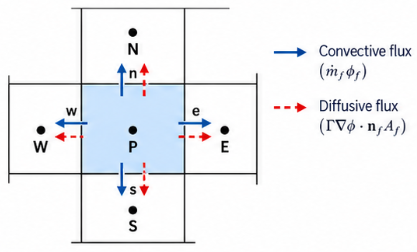
\includegraphics[\lw=.6]{media/image14.png}
\end{center}
Apply mass, momentum, energy and turbulence balances to each control volume.

\textbf{2: Approximate the face fluxes}
\begin{center}
  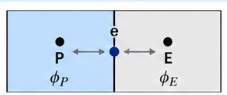
\includegraphics[\lw=.4]{media/image15.png}
\end{center}
Approximate face values from cell-centred values: use upwinding for convection and a gradient for diffusion.
\[
  \nabla \Phi_e =
  \left.\frac{\partial\Phi}{\partial x}\right|_e
  \approx \frac{\Phi_E-\Phi_P}{\Delta x_{PE}}
\]
The face flux combines convection and diffusion.

\textbf{3: Assemble the algebraic equation}
\begin{center}
  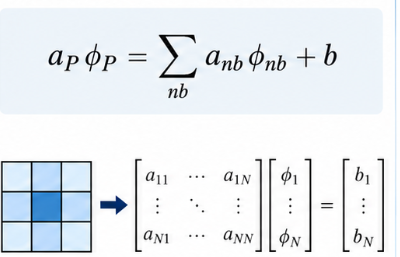
\includegraphics[\lw=.6]{media/image16.png}
\end{center}
One equation per cell forms a coupled linear system for pressure, velocity, temperature, etc. Iterate until convergence.

\section{CFD Simulation}
\subsection{Continuity equation}
\begin{gather*}
  \frac{\partial \rho \u{u}}{\partial t} + \nabla \cdot \rho \u{u}\ \u{u} = -\nabla p + \nabla\cdot \u{\u{\tau}}\\
  \frac{\partial \rho}{\partial t} + \nabla\cdot\left(\rho\u{u}\right) = 0
\end{gather*}

\subsubsection{Density based}
\[
  p = \rho R T
\]
\begin{center}
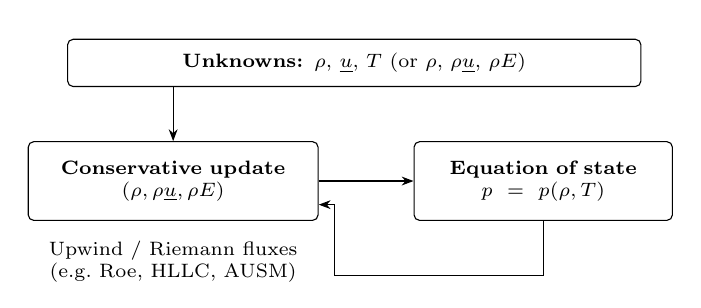
\begin{tikzpicture}[
  box/.style={draw, rounded corners=2pt, align=center,
    font=\scriptsize, inner sep=4pt, minimum height=1cm},
  flow/.style={-{Stealth[length=1.5mm]}, thin}
]
  \node[box, text width=7cm, minimum height=0.6cm] (unknowns) at (0,1.5)
    {\textbf{Unknowns:} $\rho$, $\u{u}$, $T$
      (or $\rho$, $\rho\u{u}$, $\rho E$)};
  \node[box, text width=3.4cm] (update) at (-2.3,0)
    {\textbf{Conservative update}\\$(\rho,\rho\u{u},\rho E)$};
  \node[box, text width=3cm] (eos) at (2.4,0)
    {\textbf{Equation of state}\\$p=p(\rho,T)$};
  \node[align=center, font=\scriptsize, anchor=north] at (-2.3,-0.65)
    {Upwind / Riemann fluxes\\(e.g.\ Roe, HLLC, AUSM)};

  \draw[flow] (-2.3,1.2) -- (update.north);
  \draw[flow] (update.east) -- (eos.west);
  \draw[flow] (eos.south) -- (2.4,-1.2)
    -- (-0.25,-1.2) -- (-0.25,-0.3) -- (-0.45,-0.3);
\end{tikzpicture}
\end{center}

\newcolumn
\subsubsection{Pressure based}
\[
  \nabla\cdot\u{u} = 0
\]
\begin{center}
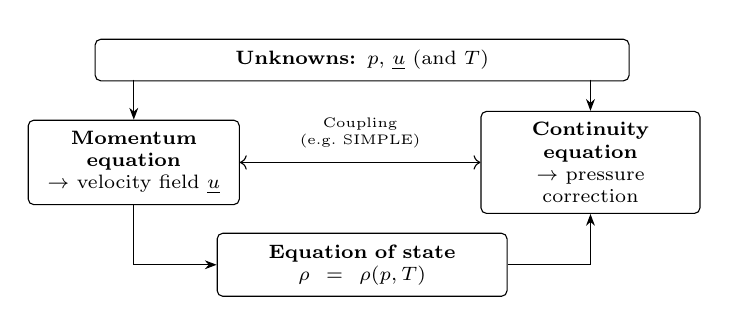
\begin{tikzpicture}[
  box/.style={draw, rounded corners=2pt, align=center,
    font=\scriptsize, inner sep=4pt, minimum height=0.8cm},
  flow/.style={-{Stealth[length=1.5mm]}, thin}
]
  \node[box, text width=6.5cm, minimum height=0.5cm] (unknowns) at (0,1.3)
    {\textbf{Unknowns:} $p$, $\u{u}$ (and $T$)};
  \node[box, text width=2.4cm] (momentum) at (-2.9,0)
    {\textbf{Momentum equation}\\$\rightarrow$ velocity field $\u{u}$};
  \node[box, text width=2.5cm] (continuity) at (2.9,0)
    {\textbf{Continuity equation}\\$\rightarrow$ pressure correction};
  \node[box, text width=3.4cm] (eos) at (0,-1.3)
    {\textbf{Equation of state}\\$\rho=\rho(p,T)$};

  \draw[flow] (-2.9,1.05) -- (momentum.north);
  \draw[flow] (2.9,1.05) -- (continuity.north);
  \draw[flow, <->] (momentum.east) -- (continuity.west)
    node[midway, above=2pt, font=\tiny, align=center]
      {Coupling\\(e.g.\ SIMPLE)};
  \draw[flow] (momentum.south) |- (eos.west);
  \draw[flow] (eos.east) -| (continuity.south);
\end{tikzpicture}
\end{center}

\subsection{Segregated vs. Coupled solution methods}
\subsubsection{Segregated method (OpenFOAM, Fluent)}
Solve for $\partial p$ :
\[
  a_c^p p_c + \sum_{nb} a_{nb}^p p_{nb} = b_c^p
\]
Solve for $\partial u$ :
\[
\begin{aligned}
  a_c^{u_x}u_{x,c} + \sum_{nb}a_{nb}^{u_x}u_{x,nb} &= b_c^{u_x}\\
  a_c^{u_y}u_{y,c} + \sum_{nb}a_{nb}^{u_y}u_{y,nb} &= b_c^{u_y}\\
  a_c^{u_z}u_{z,c} + \sum_{nb}a_{nb}^{u_z}u_{z,nb} &= b_c^{u_z}
\end{aligned}
\]

\begin{itemize}
  \item Iterative coupling; often needs underrelaxation and converges slowly.
  \item Sometimes preferable for transient simulations.
  \item Fluent: switch between segregated and coupled methods.
\end{itemize}

\subsubsection{Coupled formulation (CFX, Fluent)}
\begin{itemize}
  \item Assembles all four equations in a single coefficient matrix
\end{itemize}
\[
\begin{gathered}
  \begin{array}{r}
    \text{Momentum in }x\\
    \text{Momentum in }y\\
    \text{Momentum in }z\\
    \text{Continuity}
  \end{array}
  \;\rightarrow\;
  \underbrace{
    \begin{bmatrix}
      a_c^{uu} & a_c^{uv} & a_c^{uw} & a_c^{up}\\
      a_c^{vu} & a_c^{vv} & a_c^{vw} & a_c^{vp}\\
      a_c^{wu} & a_c^{wv} & a_c^{ww} & a_c^{wp}\\
      a_c^{pu} & a_c^{pv} & a_c^{pw} & a_c^{pp}
    \end{bmatrix}
  }_{A_c}
  \underbrace{
    \begin{pmatrix}u_c\\v_c\\w_c\\p_c\end{pmatrix}
  }_{x_c}
  +\\
  \sum_{nb=0;\,nb\ne c}^{N}
  \underbrace{
    \begin{bmatrix}
      a_{nb}^{uu} & a_{nb}^{uv} & a_{nb}^{uw} & a_{nb}^{up}\\
      a_{nb}^{vu} & a_{nb}^{vv} & a_{nb}^{vw} & a_{nb}^{vp}\\
      a_{nb}^{wu} & a_{nb}^{wv} & a_{nb}^{ww} & a_{nb}^{wp}\\
      a_{nb}^{pu} & a_{nb}^{pv} & a_{nb}^{pw} & a_{nb}^{pp}
    \end{bmatrix}
  }_{A_{nb}}
  \underbrace{
    \begin{pmatrix}u_{nb}\\v_{nb}\\w_{nb}\\p_{nb}\end{pmatrix}
  }_{x_{nb}}
  =
  \underbrace{
    \begin{pmatrix}b_c^u\\b_c^v\\b_c^w\\b_c^p\end{pmatrix}
  }_{b_c}
\end{gathered}
\]
\begin{itemize}
  \item Can become memory expensive
  \item Requires more care in implementation
\end{itemize}

\newcolumn
\section{Turbolence modeling}
\subsection{Turbolent flow development}
\subsubsection{Reynolds number}
\[
  Re = \frac{\rho U L}{\mu} = \frac{U L}{\nu}
\]
\begin{itemize}
  \item Compares inertial and viscous effects.
  \item Mainly used for forced-convection flows.
\end{itemize}

\subsubsection{Grashof number}
\[
  Gr = \frac{g\beta\Delta T L^3}{\nu^2}
\]
\begin{itemize}
  \item Compares buoyancy and viscous effects.
  \item Important for natural-convection flows.
\end{itemize}

\subsubsection{Rayleigh number}
\[
  Ra = Gr\,Pr
\]
\begin{itemize}
  \item Often used for transition in buoyancy-driven heat transfer.
\end{itemize}

\subsubsection{Typical transition criteria}
\begingroup
\scriptsize
\setlength{\tabcolsep}{3pt}
\renewcommand{\arraystretch}{1.2}
\noindent
\begin{tabularx}{\linewidth}{|>{\raggedright\arraybackslash}p{2.1cm}|c|>{\raggedright\arraybackslash}X|}
  \hline
  \textbf{Flow type} & \textbf{Criterion} & \textbf{Typical onset}\\
  \hline
  Pipe flow & $Re_D$ & Laminar below $2300$; transition $\sim 2300$--$4000$; turbulence above $4000$.\\
  \hline
  Flat-plate boundary layer & $Re_x$ & $\sim 5\times 10^5$\\
  \hline
  Cylinder wake & $Re_D$ & Vortex shedding around $47$; transition to a turbulent wake much later.\\
  \hline
  Natural convection along a vertical plate & $Ra_x$ & Often around $Ra_x>10^9$.\\
  \hline
\end{tabularx}
\par
\endgroup

\subsection{Intertial subrange}
Between large eddies and dissipative eddies, the spectrum depends only on the transfer rate $\epsilon$ and the wavenumber $k$.
\[E(k) = C_K \epsilon^{2/3} k^{-5/3}\quad , \quad C_K \approx 1.5\]

\subsection{Kolmogorov scale}
The far right of the spectrum, where viscosity finally acts.
\[\eta = \left(\frac{\nu^3}{\epsilon}\right)^{1/4}\]

where:
\begin{tabularx}{\linewidth}{ll}
  $\eta$ & smallest eddy size [m]\\
  $\nu$ & kinematic viscosity [m$^2$/s]\\
  $\epsilon$ & dissipation rate of kin. energy [m$^2$/s$^3$]
\end{tabularx}

\subsection{Turbolent kinetic energy and the three ranges}
\[k = \integral[0][\infty][E(k)][k]\]
The area under the spectrum is $k$

\begin{center}
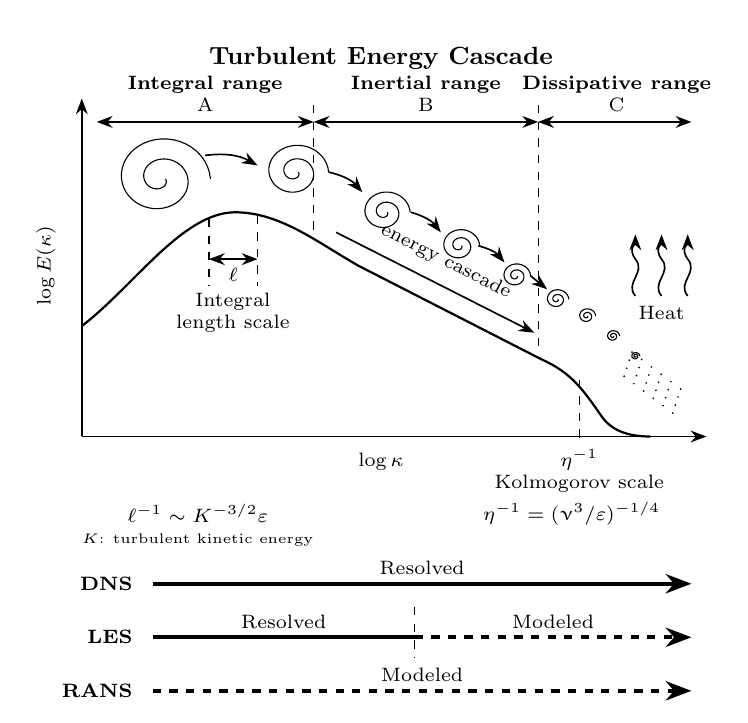
\begin{tikzpicture}[
  x=0.95cm, y=0.85cm,
  font=\scriptsize,
  >=Stealth,
  every node/.style={align=center},
  spectrum range arrow/.style={<->, semithick},
  cascade/.style={->, semithick}
]
  \node[font=\small\bfseries] at (4,5.65) {Turbulent Energy Cascade};

  % Spectral ranges.
  \node at (1.65,5.12) {\textbf{Integral range}\\A};
  \node at (4.6,5.12) {\textbf{Inertial range}\\B};
  \node at (7.15,5.12) {\textbf{Dissipative range}\\C};
  \draw[spectrum range arrow] (0.2,4.7) -- (3.1,4.7);
  \draw[spectrum range arrow] (3.1,4.7) -- (6.1,4.7);
  \draw[spectrum range arrow] (6.1,4.7) -- (8.15,4.7);
  \draw[dashed, thin] (3.1,4.95) -- (3.1,2.95);
  \draw[dashed, thin] (6.1,4.95) -- (6.1,1.25);

  % Energy spectrum and logarithmic axes.
  \draw[->, semithick] (0,0) -- (8.35,0);
  \draw[->, semithick] (0,0) -- (0,5.05);
  \node[rotate=90] at (-0.48,2.55) {$\log E(\kappa)$};
  \node at (4,-0.38) {$\log\kappa$};
  \draw[thick]
    (0,1.65) .. controls (0.7,2.25) and (1.35,3.35) .. (2.05,3.35)
    .. controls (2.65,3.35) and (3.15,2.9) .. (3.7,2.55)
    -- (6.15,1.15)
    .. controls (6.55,0.95) and (6.7,0.7) .. (6.95,0.3)
    .. controls (7.1,0.06) and (7.35,0) .. (7.6,0);

  % Eddies shrink as energy passes to higher wavenumbers.
  \foreach \cx/\cy/\rad in {
    1.05/3.85/0.67, 2.85/3.95/0.45, 4.05/3.35/0.34,
    5.05/2.85/0.27, 5.8/2.4/0.2, 6.35/2.05/0.16,
    6.75/1.8/0.12, 7.1/1.5/0.09, 7.4/1.2/0.06}
  {
    \draw[thin, domain=0:720, samples=90, variable=\t]
      plot ({\cx+\rad*(1-\t/800)*cos(\t)},
            {\cy+\rad*(1-\t/800)*sin(\t)});
  }
  \draw[cascade] (1.65,4.2) to[bend left=18] (2.35,4.05);
  \draw[cascade] (3.3,3.95) to[bend left=18] (3.75,3.65);
  \draw[cascade] (4.4,3.35) to[bend left=18] (4.8,3.05);
  \draw[cascade] (5.3,2.85) to[bend left=18] (5.65,2.6);
  \draw[cascade] (6,2.4) -- (6.22,2.2);
  \draw[cascade] (3.4,3.05) -- (6.05,1.55)
    node[midway, sloped, above=2pt] {energy cascade};
  \foreach \i in {0,...,5} {
    \foreach \j in {0,...,3} {
      \fill ({7.25+0.13*\i+0.035*\j},
             {0.9-0.11*\i+0.12*\j}) circle[radius=0.012cm];
    }
  }

  % Integral and Kolmogorov scales.
  \draw[dashed, thin] (1.7,3.25) -- (1.7,2.25);
  \draw[dashed, thin] (2.35,3.3) -- (2.35,2.25);
  \draw[spectrum range arrow] (1.7,2.65) -- (2.35,2.65)
    node[midway, below] {$\ell$};
  \node at (2.02,1.85) {Integral\\length scale};
  \draw[dashed, thin] (6.65,0.85) -- (6.65,-0.1);
  \node[below] at (6.65,-0.05) {$\eta^{-1}$};
  \node at (6.65,-0.7) {Kolmogorov scale};
  \node at (1.55,-1.15) {$\ell^{-1}\sim K^{-3/2}\varepsilon$};
  \node at (6.55,-1.15) {$\eta^{-1}=(\nu^3/\varepsilon)^{-1/4}$};
  \node[font=\tiny] at (1.55,-1.55) {$K$: turbulent kinetic energy};

  % Small-scale dissipation into heat.
  \node at (7.75,1.85) {Heat};
  \foreach \hx in {7.4,7.75,8.1} {
    \draw[cascade] (\hx,2.1)
      .. controls ({\hx-0.15},2.3) and ({\hx+0.15},2.45) .. (\hx,2.65)
      .. controls ({\hx-0.1},2.8) and (\hx,2.9) .. (\hx,3.02);
  }

  % Resolved and modeled portions of the turbulent spectrum.
  \node[anchor=east, font=\scriptsize\bfseries] at (0.8,-2.2) {DNS};
  \draw[->, line width=1.4pt] (0.95,-2.2) -- (8.15,-2.2);
  \node[above] at (4.55,-2.2) {Resolved};

  \node[anchor=east, font=\scriptsize\bfseries] at (0.8,-3) {LES};
  \draw[line width=1.4pt] (0.95,-3) -- (4.45,-3);
  \draw[->, dashed, line width=1.4pt] (4.45,-3) -- (8.15,-3);
  \draw[dashed, thin] (4.45,-2.55) -- (4.45,-3.3);
  \node[above] at (2.7,-3) {Resolved};
  \node[above] at (6.3,-3) {Modeled};

  \node[anchor=east, font=\scriptsize\bfseries] at (0.8,-3.8) {RANS};
  \draw[->, dashed, line width=1.4pt] (0.95,-3.8) -- (8.15,-3.8);
  \node[above] at (4.55,-3.8) {Modeled};
\end{tikzpicture}
\end{center}

\subsection{DNS, LES, and RANS}
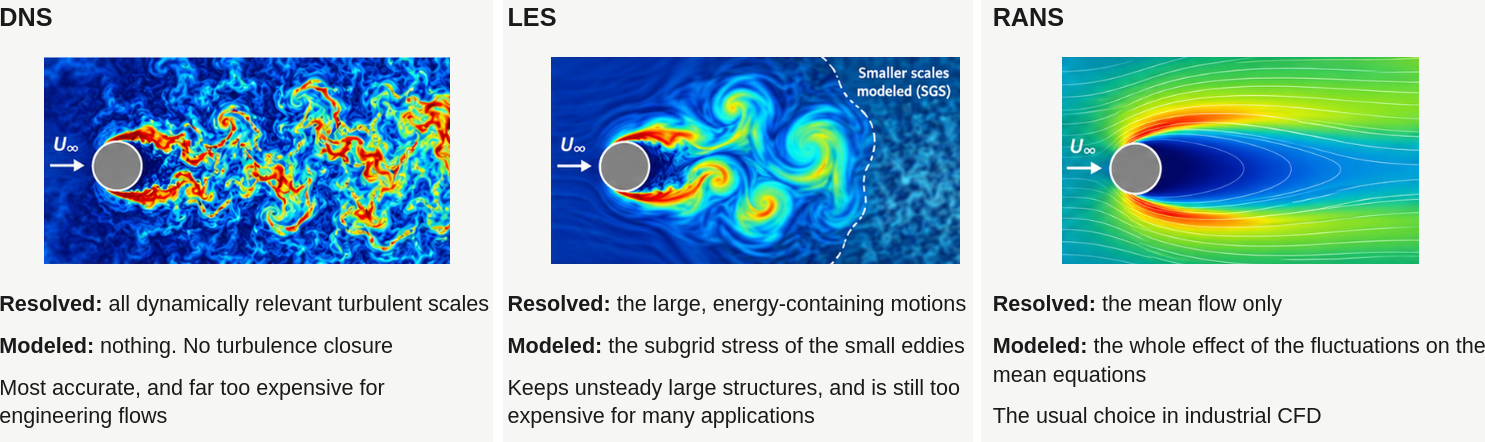
\includegraphics[\lw]{media/model-resolution.png}

\subsubsection{Reynolds-averaged Navier Stokes (RANS)}
Ensemble averaging extracts the mean from instantaneous flow properties:
\[
  \underbrace{u_i(x,t)}_{\text{instantaneous}}
  = \underbrace{\overline{u_i}(x,t)}_{\text{average}}
  + \underbrace{u_i'(x,t)}_{\text{fluctuation}}
\]
For incompressible flow with constant $\rho$ and $\mu$, pressure and viscous stress are linear and average without a new unknown. Only the convective term is nonlinear.

\textbf{1. Instantaneous momentum}
\[
  \rho\left(
    \frac{\partial u_i}{\partial t}
    + \underbrace{u_j\frac{\partial u_i}{\partial x_j}}_{\text{nonlinear}}
  \right)
  = -\frac{\partial p}{\partial x_i}
    + \mu\frac{\partial^2 u_i}{\partial x_j\partial x_j}
\]

\textbf{2. Decompose the product and average}
\[
\begin{aligned}
  u_i &= \overline{u_i}+u_i',\\
  u_i u_j &= \overline{u_i}\,\overline{u_j}
    + \overline{u_i}u_j' + u_i'\overline{u_j} + u_i'u_j',\\
  \overline{u_i u_j} &= \overline{u_i}\,\overline{u_j}
    + \overline{u_i'u_j'}
\end{aligned}
\]

The cross terms vanish because $\overline{u_i'}=0$.

\textbf{3. Averaged momentum}
\[
  \rho\left(\frac{\partial\overline{u_i}}{\partial t} + \overline{u_j}\frac{\partial\overline{u_i}}{\partial x_j}\right) = -\frac{\partial\overline{p}}{\partial x_i} + \mu\frac{\partial^2\overline{u_i}}{\partial x_j\partial x_j} \quad -\underbrace{\frac{\partial}{\partial x_j} \left(\rho\overline{u_i'u_j'}\right)}_{\text{Reynolds stress}}
\]
\[
  \tau_{ij}^{R}=-\rho\overline{u_i'u_j'}
\]

In 3D, this symmetric tensor has six independent components, but there are only three momentum equations.

Eddy-viscosity models (EVM) provide closure, e.g.\ $k$--$\epsilon$, $k$--$\omega$ and SST.

\subsection{Modeling strategies}
\subsubsection{Eddy-viscosity models (EVM)}
The six unknown stresses are related to the mean strain, as for a viscous stress.

\textbf{Boussinesq hypothesis}
\[
  \tau_{ij}^{R}=-\rho\overline{u_i'u_j'}
  =2\mu_t S_{ij}-\frac{2}{3}\rho k\delta_{ij}
\]
\begin{itemize}
  \item $2\mu_t S_{ij}$ aligns the deviatoric stress with the mean strain
  \item $\frac{2}{3}\rho k\delta_{ij}$ is the isotropic normal-stress contribution
  \item $\delta_{ij}$ is the identity tensor
\end{itemize}
\[
  S_{ij}=\frac{1}{2}\left(
    \frac{\partial\overline{u_i}}{\partial x_j}
    +\frac{\partial\overline{u_j}}{\partial x_i}
  \right),
  \qquad k=\frac{1}{2}\overline{u_i'u_i'}
\]

$S_{ij}$ is the mean strain rate and $k$ the turbulent kinetic energy per unit mass.

The eddy viscosity $\mu_t$ is modeled, not a fluid property:
\begin{itemize}
  \item One equation: Spalart--Allmaras.
  \item Two equations: $k$--$\epsilon$, $k$--$\omega$, SST.
\end{itemize}

\textbf{EVM: Two-equation models}
\begin{itemize}
  \item Common turbulence models, widely used in industry.
  \item Two additional transport equations are solved iteratively.
  \item Usually solve for turbulent kinetic energy $k$ and either dissipation rate $\epsilon$ or specific dissipation rate $\omega$.
\end{itemize}

\newcolumn
\textbf{Turbulent kinetic energy}
\[
  k\equiv\frac{\overline{u_i'u_i'}}{2}
\]
Kinetic energy per unit mass of turbulent fluctuations, mainly contained in the large eddies.

\textbf{Dissipation rate of turbulent kinetic energy}
\[
  \epsilon\equiv\nu\overline{
    \frac{\partial u_i'}{\partial x_j}
    \left(\frac{\partial u_i'}{\partial x_j}
    +\frac{\partial u_j'}{\partial x_i}\right)}
\]
Rate at which turbulent kinetic energy is converted into heat per unit mass, predominantly at the smallest eddies.

\textbf{Specific dissipation rate, or turbulent frequency}
\[
  \omega\equiv\frac{\epsilon}{C_\mu k},
  \qquad C_\mu=0.09
\]
Dissipation rate per unit turbulent kinetic energy, scaled by $1/C_\mu$; an inverse turbulent time scale with units $\mathrm{s}^{-1}$.

\subsubsection{Reynolds-stress models (RSM)}
\[
  -\rho\overline{u_i'u_j'}=
  \begin{bmatrix}
    \tau_{11}^{R} & \tau_{12}^{R} & \tau_{13}^{R}\\
    \tau_{21}^{R} & \tau_{22}^{R} & \tau_{23}^{R}\\
    \tau_{31}^{R} & \tau_{32}^{R} & \tau_{33}^{R}
  \end{bmatrix}
\qquad
\vcenter{\hbox{%
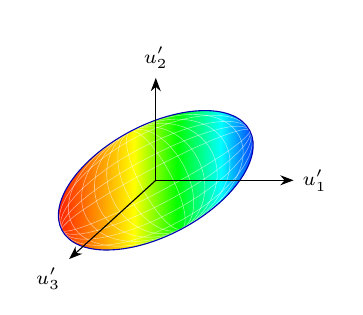
\begin{tikzpicture}[>=Stealth, font=\scriptsize]
  % Schematic anisotropic fluctuation ellipsoid.
  \pgfdeclarehorizontalshading{rsmSpectrum}{100bp}{
    color(0bp)=(red); color(25bp)=(red);
    color(35bp)=(orange); color(45bp)=(yellow);
    color(55bp)=(green); color(65bp)=(cyan);
    color(75bp)=(blue); color(100bp)=(blue)}
  \begin{scope}[rotate=28]
    \shade[shading=rsmSpectrum] (0,0)
      ellipse[x radius=1.35cm,y radius=0.7cm];
    \foreach \rsmRadius in {0.2,0.4,0.6,0.8,1.0,1.2} {
      \draw[white, opacity=0.55, very thin] (0,0)
        ellipse[x radius=\rsmRadius cm,y radius=0.7cm];
    }
    \foreach \rsmRadius in {0.15,0.3,0.45,0.6} {
      \draw[white, opacity=0.55, very thin] (0,0)
        ellipse[x radius=1.35cm,y radius=\rsmRadius cm];
    }
    \draw[blue!70!black, thin] (0,0)
      ellipse[x radius=1.35cm,y radius=0.7cm];
  \end{scope}
  \draw[->] (0,0) -- (1.75,0) node[right] {$u_1'$};
  \draw[->] (0,0) -- (0,1.3) node[above] {$u_2'$};
  \draw[->] (0,0) -- (-1.1,-1) node[below left] {$u_3'$};
\end{tikzpicture}
}}
\]
The stress is not forced to follow $S_{ij}$.\\
Each independent component has its own transport equation.
\begin{itemize}
  \item Symmetric $\u{\u{\tau}}$: six unknowns, six stress transport equations.
  \item Can represent turbulence anisotropy.
  \item More computationally demanding.
\end{itemize}

\textbf{Both approaches close the RANS equations:}\\
EVM models $\mu_t$; RSM transports the six stresses.

\subsection{Final Reynolds-averaged momentum equations under EVM}
\textbf{1. Averaged momentum, Reynolds stress still unknown}
\[
  \frac{\partial\rho u_i}{\partial t}
  +\nabla\cdot(\rho u_i u_j)
  =-\nabla p
  +\nabla\cdot\left[\mu\left(\nabla u_i+\nabla u_i^T\right)\right]
  -\nabla\cdot\left(\rho\overline{u_i'u_j'}\right)
\]

\textbf{2. Insert the Boussinesq relation}
\[
  -\rho\overline{u_i'u_j'}
  =2\mu_t S_{ij}-\frac{2}{3}\rho k I_{ij}
  =\mu_t\left(\nabla u_i+\nabla u_i^T\right)
  -\frac{2}{3}\rho k I_{ij}
\]
Because $2S_{ij}=\nabla u_i+\nabla u_i^T$, the strain term has the same form as the viscous stress, so $\mu_t$ adds to $\mu$.

\textbf{3. Momentum equation under EVM}
{\footnotesize\[
  \frac{\partial\rho u_i}{\partial t}
  +\nabla\cdot(\rho u_i u_j)
  =-\nabla p
  +\nabla\cdot\left[(\mu+\mu_t)\left(\nabla u_i+\nabla u_i^T\right)\right]
  -\nabla\cdot\left(\frac{2}{3}\rho k I_{ij}\right)
\]}

Effective viscosity is the sum of physical and modeled viscosity:
\[
  \mu_{\mathrm{eff}}=\mu+\mu_t
\]

















































































\end{multicols*}
\end{document}
